\section{El modelo estándar de la física de partículas}

\begin{frame}{La física de partículas elementales}
    \begin{block}{Modelo Estándar}
        El modelo estándar de la física de partículas es una teoría de la física que explica tres de las cuatro fuerzas fundamentales de la naturaleza; estas son las interacciones electromagnética, fuerte y débil. En ella se considera que todo está hecho de tres tipos de partículas elementales: leptones, quarks y mediadores. \cite{griffiths2020introduction}
    \end{block}
\end{frame}

\begin{frame}{Tabla de las partículas elementales}
    \begin{figure}
        \centering
        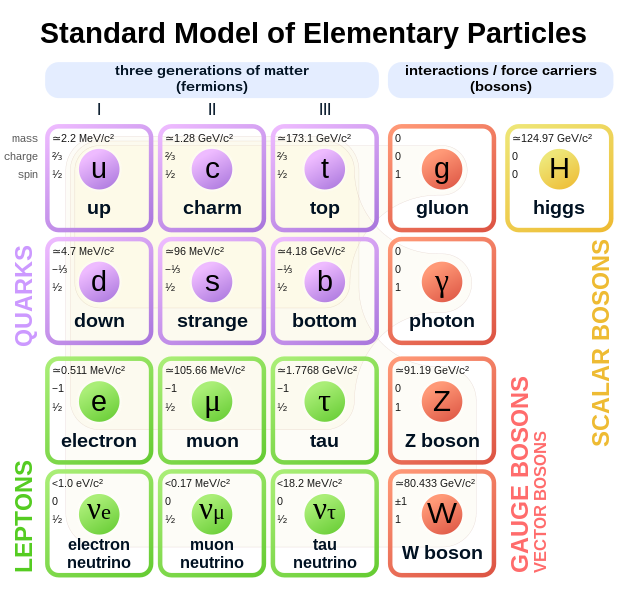
\includegraphics[scale=0.28]{pic/Standard_Model_of_Elementary_Particles.svg.png}
        \caption{En esta tabla se clasifican las partículas elementales en leptones, quarks y mediadores.}
        \label{fig:particles_table}
    \end{figure}
\end{frame}

\subsection{El modelo de Quarks}

\begin{frame}{Los Quarks}
    \begin{block}{Tipos de Quarks}
        Nosotros nos concetramos en los quarks, la física de partículas considera seis distintos "sabores" de quarks que son caracterizados por los siguientes términos.
    \end{block}
    \begin{table}[h]
        \centering
        \begin{adjustbox}{max width=\textwidth}
          \begin{tabular}{c|c|c|c|c|c|c|c|c}
            Quark &  Generación & Carga Q & Downess D & Upness U & Strangeness S & Charm C & Beauty B & Truth T\\
            \hline
            Down d    & Primera & -1/3 & -1 & 0 & 0  & 0 & 0  & 0 \\
            Up u      & Primera & 2/3  & 0  & 1 & 0  & 0 & 0  & 0 \\
            Strange s & Segunda & -1/3 & 0  & 0 & -1 & 0 & 0  & 0 \\
            Charm c   & Segunda & 2/3  & 0  & 0 & 0  & 1 & 0  & 0 \\
            Bottom b  & Tercera & -1/3 & 0  & 0 & 0  & 0 & -1 & 0 \\
            Top t     & Tercera & 2/3  & 0  & 0 & 0  & 0 & 0  & 1 
        \end{tabular}
        \end{adjustbox}
    \end{table}
    
    Cada a cada una de las partículas de la tabla le corresponde un \textbf{antipartícula} con los signos contrarios.
    
\end{frame}

\subsection{Mesones y bariones}

\begin{frame}{Reglas de composición}

    Los quarks no se encuentran solos en la naturaleza, siempre están confinados en grupos, pero estos no se agrupan en cualquier configuración. Obedecen a las siguientes reglas: 
    
    \begin{columns}
    \begin{column}{0.5\textwidth}
       \begin{tcolorbox}[colback=blue!5!white, colframe =blue!75!black, title=Mesones]
            Cada mesón está compuesto de un quark y un antiquark.
        \end{tcolorbox}
    \end{column}
    \begin{column}{0.5\textwidth}  
        \begin{center}
             \begin{tcolorbox}[colback=blue!5!white, colframe =blue!75!black, title=Bariones]
                Cada barión está compuesto de tres quarks, y un antibarión de tres antiquarks.
            \end{tcolorbox}
         \end{center}
    \end{column}
    \end{columns}
\end{frame}

\subsection{Quarkonium}

\begin{frame}{Quarkoniums o quarkonios}
    \begin{tcolorbox}[colback=blue!5!white, colframe =blue!75!black, title=Definición]
        Un quarkonium (o quarkonio como se le suele llamar en español) es un tipo particular de mesón que:
        está compuesto por un quark y (estrictamente) su antiquark, no tiene sabor.
    \end{tcolorbox}
\end{frame}

\begin{frame}{Ejemplos de quarkoniums}

    \begin{columns}
    \begin{column}{0.5\textwidth}
       \begin{tcolorbox}[colback=blue!5!white, colframe =blue!75!black, title= Charmonium]
            También llamado mesón $J / \Psi $, está formado por un quark charm y su antipartícula, fue descubierta en 1974.
            Tiene una masa promedio de  $ 3.0969 GeV/c^2 $ y una vida media de $7.2X10^{-21} s$.
        \end{tcolorbox}
    \end{column}
    \begin{column}{0.5\textwidth}  
        \begin{center}
             \begin{tcolorbox}[colback=blue!5!white, colframe =blue!75!black,title= Bottonium]
                También llamado mesón $ \Upsilon $, está formado por un quark bottom y su antipartícula, fue descubierta en 1977.
                Tiene una masa promedio de  $ 9.46 GeV/c^2 $ y una vida media de $1.21X10^{-20} s$.
            \end{tcolorbox}
         \end{center}
    \end{column}
    \end{columns}
\end{frame}






